
%%%%%%%%%%%%%%%%%%%%%%% file typeinst.tex %%%%%%%%%%%%%%%%%%%%%%%%%
%
% This is the LaTeX source for the instructions to authors using
% the LaTeX document class 'llncs.cls' for contributions to
% the Lecture Notes in Computer Sciences series.
% http://www.springer.com/lncs       Springer Heidelberg 2006/05/04
%
% It may be used as a template for your own input - copy it
% to a new file with a new name and use it as the basis
% for your article.
%
% NB: the document class 'llncs' has its own and detailed documentation, see
% ftp://ftp.springer.de/data/pubftp/pub/tex/latex/llncs/latex2e/llncsdoc.pdf
%
%%%%%%%%%%%%%%%%%%%%%%%%%%%%%%%%%%%%%%%%%%%%%%%%%%%%%%%%%%%%%%%%%%%


\documentclass[runningheads,a4paper]{llncs}

\usepackage{amssymb}
\setcounter{tocdepth}{3}
\usepackage{graphicx}


\usepackage{url}
\urldef{\mailsa}\path|{alfred.hofmann, ursula.barth, ingrid.haas, frank.holzwarth,|
\urldef{\mailsb}\path|anna.kramer, leonie.kunz, christine.reiss, nicole.sator,|
\urldef{\mailsc}\path|erika.siebert-cole, peter.strasser, lncs}@springer.com|    
\newcommand{\keywords}[1]{\par\addvspace\baselineskip
\noindent\keywordname\enspace\ignorespaces#1}

\begin{document}

\mainmatter  % start of an individual contribution

% first the title is needed
\title{Energy Aggregation using Product of HMMs}

% a short form should be given in case it is too long for the running head
%\titlerunning{Lecture Notes in Computer Science: Authors' Instructions}

% the name(s) of the author(s) follow(s) next
%
% NB: Chinese authors should write their first names(s) in front of
% their surnames. This ensures that the names appear correctly in
% the running heads and the author index.
%

\author{Megha Gupta\inst{1} \and Haimonti Dutta\inst{2}
\thanks{The author is also affiliated to the Institute of Data Science and Engineering (IDSE), Columbia University and is an adjunct professor at IIIT-Delhi.}
Ullas Nambiar\inst{3} \and Amarjeet Singh\inst{4}}

\institute{IIIT Delhi, India,\\
\email{meghag@iiitd.ac.in},\\ 
%WWW home page:
%\texttt{http://users/\homedir iekeland/web/welcome.html}
\and
State University of New York, Buffalo,\\
haimonti@buffalo.edu\\
%\thanks{The author is also affiliated to the Institute of Data Science and Engineering (IDSE), Columbia University and is an adjunct professor at IIIT-Delhi.}%
\and
EMC, India \\
Ullas.Nambiar@emc.com\\
\and
IIIT Delhi, India\\
amarjeet@iiitd.ac.in
}

%\author{Megha Gupta\\
%\institute{IIIT Delhi,\\
%\email{meghag@iiitd.ac.in\\
%%\thanks{Please note that the LNCS Editorial assumes that all authors have used
%%the western naming convention, with given names preceding surnames. This determines
%%the structure of the names in the running heads and the author index.}%
%\and Haimonti Dutta
%\institute{State University of New York,Buffalo,\\
%\email{haimonti@buffalo.edu\\
%\and Ullas Nambiar
% \and Amarjeet Singh}
%}
%}}}
%Anna Kramer\and Leonie Kunz\and Christine Rei\ss\and\\
%Nicole Sator\and Erika Siebert-Cole\and Peter Stra\ss er}
%
\authorrunning{Energy Aggregation using Product of HMMs}
% (feature abused for this document to repeat the title also on left hand pages)

% the affiliations are given next; don't give your e-mail address
% unless you accept that it will be published

%
%\institute{IIIT Delhi, India,\\
%State University of New York, Buffalo
%Tiergartenstr. 17, 69121 Heidelberg, Germany\\
%\mailsa\\
%\mailsb\\
%\mailsc\\
%\url{http://www.springer.com/lncs}}

%\institute{IIIT Delhi,\\
%\email{meghag@iiitd.ac.in}\\} 
%\institute{State University of New York, Buffalo,\\
%\email{haimonti@buffalo.edu}\\} 

%WWW home page:
%\texttt{http://users/\homedir iekeland/web/welcome.html}
%\and
%Universit\'{e} de Paris-Sud,
%Laboratoire d'Analyse Num\'{e}rique, B\^{a}timent 425,\\
%F-91405 Orsay Cedex, France}


%
% NB: a more complex sample for affiliations and the mapping to the
% corresponding authors can be found in the file "llncs.dem"
% (search for the string "\mainmatter" where a contribution starts).
% "llncs.dem" accompanies the document class "llncs.cls".
%

%\toctitle{Lecture Notes in Computer Science}
%\tocauthor{Authors' Instructions}
\maketitle


\begin{abstract}
Real time spatio-temporal energy consumption data is captured by large scale deployment of smart meters. Data from these meters are usually sent to a base station (BS) where they are aggregated for analytics. Each BS aggregates the load derived from all the meters connected to that station. The  readings received at the BS are adhoc and usually not synchronized in time. Different smart meters can send data points when they are collected resulting in inconsistent data including aggregating non-aligned time stamped readings, readings with missing values, repeated values, meter reset readings.
%The problem arises when the analytics is to be performed on the data which is aggregated from the inconsistent messages passed by all the meters connected to a particular base station.
%the demand response programs have been a cost effective alternative to meet the occasional peak demands. 
%We propose to solve the problem of energy aggregation where the constituents of each aggregate are inconsistent with respect to time. The challenges with the inconsistent data includes aggregating non-aligned time stamped readings, readings with missing values, repeated values, meter reset readings. 
We address the problem of learning from disparate data streams (with inconsistencies) by modelling streams as HMMs and the process of aggregating data at the BS as a Product of HMMs. This enables us to perform load forecasting using machine learning techniques. Empirical results are presented on two data sets - Reference Energy Disaggregation Data (REDD) and energy consumption data collected from faculty housing at IIIT-Delhi. The results show that this technique performs the best by combining via product, all the HMMs (corresponding to each data stream) with binary states (on, off or standby) and training time linear to the number of HMMs.
%We address the problem of aggregating energy data in context with the load forecasting using a machine learning technique called product of Hidden Markov Models (PoHMM). 
%The objective function used for learning is the contrastive divergence between the observed data and the reconstructed data produced by running a Gibbs sampler. 
%Data analytics in energy domain, load forecasting on aggregates of power meters, Energy aggregation problem using pohmm, The STLF accuracy improves with larger aggregates, This paper deals with the energy aggregation problems in electrical system. The challenges included problem of aggregating inconsistent data, across time, in case of electrical systems.
\keywords{We would like to encourage you to list your keywords within
the abstract section}
\end{abstract}


\section{Introduction}

Smart meters consisting of real time sensors, power outage notifications and power quality monitoring are widely used today. These meters provide a host of benefits like energy efficiency and savings, improved retail competition, better demand response actions, improved tariffs, lower bills due to better customer feedback, accurate billing, less environmental pollution, etc. \cite{Klopfert}
They generate huge amount of time series data which can be used for gaining meaningful insights through analytics.
They can measure site specific information and also help agencies set different electricity prices for consumption based on the time of the day, seasons, holidays, etc. Based on the data collected from smart meters, a feedback sent to the customers by the utilities that can help consumers better manage their resources. McKerracher et al. \cite{mckerracher} show that by providing real time feedback, consumers can reduce the consumption by 3-5\%.
%This helps consumers to better manage their energy resources and reduce their bills and carbon emissions.


In recent years, machine learning has been applied to the problem of energy consumption and demand forecasting analysis. The role of the machine learning algorithm is to study the sensor data and provide alerts and warnings when anomalous behaviour occurs or to inform (and remind) customers when certain activities were performed, which rooms they occupied, and what appliances they used most frequently during that period. This information can be transmitted to customers in timely fashion via phone, email or the Internet.
Chicco et al. \cite{1626400} compared several clustering techniques (such as hierarchical, KMeans) and observed that the hierarchical clustering and modified follow-the-leader perform best among the rest K-Means, fuzzy K-Means to group customers with similar electrical behaviour \cite{5620917}. Wijaya et al. \cite{Wijaya} used classifiers like random forest, decision trees (J48), logistic and naive bayes to identify customers with similar electricity consumption profiles.
%Sensor data collected from smart homes are used to reveal activity patterns of the residents, which can then be correlated with the total energy consumption. This enables utility companies and their customers to associate activities with energy usage and costs, devise intelligent systems to control home environments improving energy efficiency and reducing costs. Typically, sequences of usage patterns that appear frequently at different time scales (daily, weekly, monthly, yearly) and across different homes are studied and 
%%; trends of electricity consumption (steadily increasing, decreasing, cyclic, seasonal) for individual homes and across the community; and anomalies (sudden peaks or drops on consumption) for individual homes and across the community.
%outlier detection algorithms are designed to enable customers to be notified that they are consuming unusually large amount(s) of energy during some specific period. 
Related problems involve study of trends of electricity consumption (steadily increasing, decreasing, cyclic, seasonal) and sudden anomalous behaviour (sudden peaks or drops on consumption) for individual homes and across the community \cite{Diane}.

In this paper, we use Hidden Markov models (HMMs) to analyse the time series energy data.
We model the data stream from each source as a HMM with its states represented as ON/OFF.  For $N$ sources, there are $N$ HMMs and  the total number of states collectively are $2^N$. The observations represent the energy consumed in a particular state. These observations are recorded at different time scales for different sources. \\
In order to aggregate the data from all the different sources, we build a machine learning model using products of HMMs (PoHMMs) and apply it to the energy aggregation problem. There are many reasons why the product model constructed from many HMMs is appropriate. 
%First, this model is ideal for data which is caused by multiple underlying influences.
%First, this model allows each HMM to make decisions based on few dimensions without actually having to worry about covering the full dimensionality of the problem.
First, in a high-dimensional space each model constraints a different subset of dimensions but their product constraints all of the dimensions.
Second, HMMs alone are not efficient at capturing long range structure in time series \cite{Taylor} -- in contrast to PoHMMs  \cite{andrew} allow each model to remember a different piece of information about the past.
Two different proof of concepts are presented -- first one on the REDD \footnote{http://redd.csail.mit.edu/} data set and the other one on real data collected at the faculty housing in India. 
%application of are aggregating energy consumption information using a model that extends the power of HMMs. HMM's are used as the basic expert in the of product of experts model. 

%There have been some experiments on sentence and character strings modelling, factorial time series to demonstrate the advantages of using a PoHMM over an equivalently sized regular HMM}.
%We have applied the contrastive divergence learning algorithm on two datasets, REDD dataset and the faculty housing dataset which was generated by smart meters.
%The system architecture for the faculty housing dataset consists of two smart meters $S_1$ and $S_2$ installed in a faculty housing building collecting data from twelve floors. $S_1$ collects data from first six floors (0 to 5th) and $S_2$ collects data from the rest of the floors (6 to 11th). The data collected from two meters is aggregated using product of experts technique in a way that the contrastive divergence between the two probability distributions is minimized. 
%The proof of concept of REDD dataset and faculty housing dataset is given in section~\ref{sec:redd} and section~\ref{sec:faculty} respectively.

\noindent \textbf{Organization:} This paper is organized as follows: Section~\ref{related} examines related work on data analytics on aggregated data of smart meters; Section~\ref{sec:review} provides a review of products of Hidden Markov Models (HMMs) and how they relate to our application. The two proofs of concepts are introduced in Section~\ref{poc} illustrating the effectiveness of the use of product of HMMs in the energy aggregation problem. Finally, Section~\ref{conclusion} concludes the work.

\section{Related Work}
\label{related}
In this section, we describe work that uses ensemble learning techniques and non-ensemble learning techniques to solve problems in energy domain.
\subsection{Non-ensemble based learning techniques}


\noindent \textbf{Energy Aggregation}
%Devaine et al. (CITE) study ...
is a method of combining data from different sources such that several unreliable data measurements combine to produce a more accurate signal by enhancing the common signal and reducing the uncorrelated noise. As the sensor network generates lot of data for the end user to process, there are automated methods employed to aggregate data. This data fusion is generally known as data aggregation which combines the data into a set of meaningful information \cite{Heinzelman00energy}.
The sensor nodes are organised in a tree structure, called aggregation tree. The leaves of this tree are the sensor devices, the internal nodes are the aggregator devices that takes the data from the leaves, aggregates it and sends it to its parent node which is the root of the tree. \\
The main objective of data aggregation is to reduce the unnecessary information thereby reducing the network traffic and improving the privacy of the customers from internal and external entities by keeping only the necessary information \cite{taban}. 


%To study the process of energy aggregation, data is collected from multiple smart meters. This collected data is very large which in turn makes the analytics on top of it very difficult. Also, this detailed energy consumption data leads to privacy breach and other risks related to it. To address this problem, there has been work done \cite{Wijaya} to reduce the smart meter data numerosity by converting it into symbolic representation and then allowing algorithms on top of it. They have applied the symbolic representation tasks for customer segmentation and load forecasting.

%The purpose of energy aggregation is to get some valuable information about single or multi-site units. 
%This work evaluates the trend of degrading performance of the state of the art algorithms when the number of considered meters decrease \cite{BLTJ:BLTJ21650}. Short term load forecasts at the meter level help the company communicate with the customer about energy savings and billing. STLF handles prediction of one hour upto one week.
%The energy aggregation problem has been tackled in a variety of ways including topology control, energy conserving sleep scheduling, mobile data collectors and data aggregation. 
%Research has been done on the role of energy on the growth of the country's economy \cite{NYAS:NYAS5921}.

\noindent \textbf{Energy Disaggregation} or Non-intrusive appliance load monitoring (NIALM) is a process in which the household's aggregate electricity consumption is broken down into individual appliance's consumption. The motivation behind this task is twofolds; first, the reduction in energy consumption by using the information given to the household occupants about the individual appliance's electricity consumption; second, recommending the occupants to defer the use of appliance to a time of day when electricity is cheaper. Approaches for energy disaggregation from smart meter using ML techniques fall in two categories; first group is where sub-metered data is available to train appliance models prior to performing disaggregation; second group uses unsupervised disaggregation methods that require labelling of detected appliance, assuming the type and number of household appliance.
Parson et al. \cite{eps272990} proposed an approach to NIALM that separates the energy consumption of individual appliance iteratively from the aggregated load using hidden Markov models. Several studies have been done in this regard, one of the unsupervised disaggregation method \cite{DisaggregationHSMM} that outperforms other unsupervised disaggregation methods is conditional factorial hidden semi-Markov model. This model when integrated with other features, accurately represents the individual appliance energy consumption. In one of the work, Kolter et al. \cite{NIPS2010} show that by discriminately training the sparse coding algorithms using a method based on structured prediction, the performance of the algorithm significantly improves on the energy disaggregation task. In another study, Kolter et al. \cite{KolterJ12} exploits the additive structure of the FHMM to develop a convex formulation of approximate inference algorithm that achieves state-of-the-art performance in energy disaggregation problem. The work on this task is quite large, therefore doing a complete survey is out of the scope. So, we have provided the seminal references here.


\noindent \textbf{Load Forecasting} refers to the projection of electrical load required in a certain geographical area with the use of previous electrical load usage in the same area. It is extremely important for efficient power system planning and operation, energy purchasing and generation, load switching, infrastructure development. It encompasses various factors like, historical load, weather data, population, energy supply and price, time of the year, etc.
It is usually divided into three categories, short-term forecasts (one hour to one week) , medium-term forecasts (one week to one year) and long-term forecasts (more than a year).
In short term load forecast, \cite{Bakirtzis} and \cite{Chen} used a three layer feed forward artificial neural network to predict daily load profiles. In a paper by \cite{Chow}, nonlinear autoregressive integrated neural network was used to predict daily load consumption.
In medium term load forecasts, the author forecasts \cite{Falvo} the monthly load through knowledge based activities from the output of the ANN based stage providing yearly energy predictions. Similarly, in \cite{bassi}, time lagged feedforward neural network is used to do monthly forecasting on the basis of historical series of electrical load, economic and demographic variables. Also, the authors from covenant university, \cite{samuel} performed load forecasting of their own educational institute using the models based on linear, compound growth and cubic methods of regression analysis.
In long term load forecasting, study done by \cite{Daneshi} resulted in showing that the models based on regression analysis did not give very accurate predictions as compared to fuzzy neural network which performed better due to better handling with non linear systems. Another work  \cite{Zhang} uses support vector regression to derive non linear relationship between load and economic factors like GDP for long term forecasting in developing countries.



\noindent \textbf{Customer Segmentation} is the process of dividing a large homogeneous market into identifiable segments having similar demand characteristics. The appliance specific data has the potential to improve energy efficiency marketing by improving market segmentation, diversifying programs and transforming product development and evaluation \cite{CarrieArmel2013213}. This analysis is useful in various ways, like demand response system, intelligent distribution channel. The author \cite{wijaya2014consumer} segments the customers based on contextual dimensions like location, seasons, weather patterns, holidays, etc which help with various higher level applications like usage-specific tariff structure, theft detection, etc. In \cite{Albert}, author proposes to infer occupancy states from consumption time series data by using HMM framework. They investigate the effectiveness of HMM and model based cluster analysis in producing meaningful features of the classification. 
%This work suggests the dynamics of time series as captured by HMM analysis can be valuable.

\subsection{Ensemble based learning techniques}
Ensemble learning is a method where multiple learners are trained to solve the same problem. It constructs a set of hypothesis and combines them to generate the final result.
\subsubsection{Prediction with expert advice}
A study done by \cite{Shen}, proposed a Pattern Forecasting Ensemble Model (PFEM) comprising of five forecasting models using different clustering techniques, like k-means model, self-organising map model, hierarchical clustering model, k-medoids model and fuzzy c-means model. They have showed that on three real-world dataset, their proposed ensemble model outperformed all the five individual model in case of day ahead electricity demand prediction.
Another study \cite{Felice} highlighted the importance of regularised negative correlation learning ensemble methodology on the problem of energy load hourly prediction. This method tried to overcome the problem of variability in neural network due to high sensitivitiness to the initial conditions. As this method combines the outputs of several neural networks, it achieves a marked reduction in error after introducing external data. \\
An extension of HMMs, called Factorial Hidden Markov Model (FHMM) \cite{fhmm} is a class of ensemble based learning models that addresses the need for distributed hidden states in HMMs. The FHMM generalizes the HMM by representing the state using a collection, instead of single discrete variable. However, FHMMs being directed models, when conditioned on the observed sequence, the hidden state chains become independent making the inference easy but learning more complex. Thus, the exact inference becomes intractable, leaving one to resort to approximate inference techniques like Gibbs sampling or variational approximations.


%To model a complicated, high-dimensional data distributions, an approach called mixture of gaussians is widely used. In this method, each simple model which is a gaussian is combined using a weighted arithmetic mean of individual distributions. Such mixtures of tractable models can easily fit to data using expectation-maximization (EM) and are more powerful than their individual component. So, a different way of combining these distributions is by multiplying them together and then renormalizing them.
%In our paper,  we deal with the problem of energy aggregation using ensemble learning model. Each HMM is used to represent a state of an appliance. An appliance can have states like ON or OFF. The combination of the outputs from each of these HMM models gives us our ensemble based learning model, Product of Hidden Markov Model (PoHMM) \cite{hinton2000}. This learning technique outputs the probability distribution by combining the outputs from several simpler distributions. It allows each model to make a decision on the basis of few dimensions.


\begin{figure*}
\centering
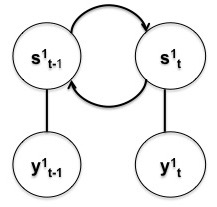
\includegraphics[width=4cm,height=3cm]{hmm1.jpg}
\label{fig:hmm1}
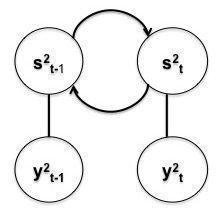
\includegraphics[width=4cm,height=3cm]{hmm2.jpg}
\label{fig:hmm2}
\caption{HMM $S^1$ and $S^2$}
\end{figure*}

\section{Review}
\label{sec:review}

%Benveniste defines HMM as a triple (\'{A}, $\mu$, $\pi$) where \'{A} = (X,$X_0$,A,T) is an automaton, $\mu$ is the initial state probability, $\pi$ is factored as state transition probability $\pi$$_{x}$ and message transition probability $\pi$$_{A}$. He uses a random arbiter $\alpha$, with values {first, second, third} to choose automaton to initiate transition. If $\alpha$ = first then first automaton chooses any transition having a private message whereas second automaton performs a stuttering transition, and vice versa for $\alpha$ = second. If $\alpha$ = both, then both automata agree on some shared message and move accordingly.

A Hidden Markov Model (HMM) is a statistical Markov model that represents the probability distribution over a sequence of observations \cite{Ghahramani}. They are found useful in applications like speech \cite{Rabiner}, handwriting, gesture recognition, part-of-speech tagging, bioinformatics, etc. It has two properties, first, the observation at time $t$, $y_{t}$ is generated by a process whose state at time $t$, $s_{t}$ is hidden from the observer and second, is that this hidden state process satisfies Markov property which states that given the value at state $s_{t-1}$, the value at current state $s_{t}$ is independent of all the states prior to $t-1$. The subscripts $i$ and superscripts $j$ indicate the model at $i$th time and the $j$th HMM. The state space of the HMM is discrete, that is a state can take $2$ values denoted by ON and OFF. The observed values represent the aggregated load/energy collected from different data streams at time $t$. In order to define probability distribution over the sequence of observation, it is important to define probability distribution over the initial state P($s_{1}$), the transition probability P($s_{t}|s_{t-1}$) and the observed probability P($y_{t}|s_{t}$) where $y_{t}$ is the observation at time $t$. \\
Following a notation in \cite{Rabiner}, HMM is composed of a 3-tuple \{A, B, $\pi$ \} where A is the transition probability, B is the observed probability and $\pi$ is the initial state probability.
%HMMs are widely used for modelling time series data. They are found useful in applications like speech, handwriting, gesture recognition, part-of-speech tagging, bioinformatics, etc.
HMMs solve three fundamental problems:
1. Given the model $\lambda$ = \{A, B, $\pi$ \}, and observation sequence Y = \{$y_{1}$,...,$y_{T}$\}, how do we efficiently compute the probability of the sequence of observations given the model, that is P($Y|\lambda$).
2. Given the model $\lambda$ and observation sequence Y, what is the underlying state sequence \{$s_{1}$,...,$s_{T}$\} that best explains the observations.
3. Given the observation Y and state space sequence S, how do we need to adjust the parameters so as to find the model $\lambda$ that maximises P($Y|\lambda$).\\
In this paper, we deal with the third problem as it involves learning parameters by training the model with the historical data and then using these parameters to predict the future observations.
The figure ~\ref{fig:hmm1} shows the HMM $S^1$ and $S^2$ generated by a data stream.

%Using the traditional HMM notation for the parameter $\lambda$ = \{A, B, $\pi$ \} where A is the transition probability, B is the observed probability and $\pi$ is the initial state probability. For HMMs, $S^{1}$ \& $S^{2}$ we have the values of A, B, $\pi$ as shown in table ~\ref{table:A}, ~\ref{table:B}, ~\ref{table:pi} respectively.

%Distributed networks can be modeled using interacting automata.
%Benveniste \cite{benveniste} defines automaton as a quadruple, \'{A} = (X,$X_0$,A,T) where X is a finite state of sets, $X_0$ is the subset of initial states, A is a finite set of messages, T is a set of transitions of the form t = \{x\_,a,x\} where x\_ is the previous state, a is the message label on which the state transitions to the next state x. The figure~\ref{fig:ex} below explains the automata with an example.\\


%For HMM R, X$_{R}$ = \{2; $R_1$,$R_2$\}, X$_{0R}$ = \{$R_1$\}, A$_{R}$ = \{a,b\}, T$_{R}$ = \{$R_1$,a,$R_1$; $R_1$,b,$R_2$; $R_2$,a,$R_2$; $R_2$,b,$R_1$\} \\
%For HMM S, X$_{S}$ = \{3; $S_1$,$S_2$,$S_3$\}, X$_{0S}$ = \{$S_1$\}, A$_{S}$ = \{a,b\}, T$_{S}$ = \{$S_1$,a,$S_1$; $S_1$,b,$S_2$; $S_2$,a,$S_2$; $S_2$,b,$S_3$; $S_3$,a,$S_3$; $S_3$,b,$S_1$\} \\
%The product of two HMMs P = R x S is defined as follows: \\
%X = X$_{R}$ x X$_{S}$ \\
%$X_0$ = X$_{0R}$ x X$_{0S}$ \\
%A = A$_{R}$ $\cup$ A$_{S}$ \\
%t = (x\_,a,x)  \\

%Benveniste uses a notion of stuttering transition which helps to distinguish between local and global time by inserting dummy transitions between two transitions of a local automaton attached to a node. This stuttering transition waits for others to progress.

%\begin{table}[h]
%\centering
%\begin{tabular}{ l | c | c }
% $A_{S^{1}}$ & $S^1_1$ & $S^1_2$ \\
%\hline
%$R_1$ & 0.6 & 0.4 \\
%$R_2$ & 0.3 & 0.7 \\
%\end{tabular}
%\quad
%\begin{tabular}{ l | c | c | c }
%  $A_{S^{2}}$ & $S^2_1$ & $S^2_2$ & $S^2_3$ \\
%\hline
%$S_1$ & 0.6 & 0.3 & 0.1 \\
%$S_2$ & 0.4 & 0.1 & 0.5 \\
%$S_3$ & 0.2 & 0.4 & 0.4 \\
%\end{tabular}
%\caption{Transition probabilities, A}
%\label{table:A}
%\end{table}
%
%\begin{table}[h]
%\centering
%\begin{tabular}{ l | c | c }
% $B_{S^{1}}$ & a & b \\
%\hline
%$S^1_1$ & 0.2 & 0.8 \\
%$S^1_2$ & 0.5 & 0.5 \\
%\end{tabular}
%\quad
%\begin{tabular}{ l | c | c | c}
% $B_{S^{2}}$ & a & b & c\\
%\hline
%$S^2_1$ & 0.2 & 0.3 & 0.5 \\
%$S^2_2$ & 0.5 & 0.4 & 0.1 \\
%$S^2_3$ & 0.4 & 0.3 & 0.3 \\
%\end{tabular}
%\caption{Observed probabilities, B}
%\label{table:B}
%\end{table}
%
%\begin{table}[h]
%\centering
%\begin{tabular}{ l | c | c }
%&  $R_1$ & $R_2$ \\
%\hline
%$\pi_{S^{1}}$ & 0.4 & 0.6 \\
%\end{tabular}
%\quad
%\begin{tabular}{ l | c | c | c}
%&  $S_1$ & $S_2$ & $S_3$\\
%\hline
%$\pi_{S^{2}}$ & 0.4 & 0.4 & 0.2 \\
%\end{tabular}
%\caption{Initial state probabilities, $\pi$}
%\label{table:pi}
%\end{table}

%Talking in terms of HMM, requires us to equip products of automata with probabilities. 

\subsection{Product of HMMs}
\label {pohmm}
PoHMM is a model that combines several HMMs by multiplying their individual distribution together and then renormalizing them. Its representation includes both directed and undirected links where the hidden states are causally connected to the other hidden states but non causally related to the visible states. This causes different conditional independence relationships among the variables in graphical model. 
%It is a way of combining HMM's to form distributed state time series model. It is defined by multiplying together the densities of its, k experts and renormalizing them. 
The figure~\ref{fig:product} is a product of two HMMs P = $S^1$ x $S^2$ where the superscript in $S^1$ indicates the kth HMM. The number of states in the PoHMM is the product of states in $S^1$ and $S^2$ which is $4$ in our case. The connections formed in the P depend on the links in the multiplying HMMs. 
%The resultant HMM will have a pair (s,s) X = \{6; $R_1$$S_1$, $R_1$$S_2$, $R_1$$S_3$, $R_2$$S_1$, $R_2$$S_2$, $R_2$$S_3$\} \\
%$X_0$ = \{$R_1$$S_1$\} \\
%A = \{a,b\} \\


%The rules for synchronised product construction are : \\
%1. $<p,q>$ --a--$>$ $<p',q>$ if a $\in$ A$_{R}$ $\cap$ A$_{S}$ and p --a--$>$ p' and q --a--$>$ q'	\\
%2. $<p,q>$ --a--$>$ $<p',q>$ if a $\in$ A$_{R}$, a $\notin$ A$_{S}$ and p --a--$>$ p'	\\
%3. $<p,q>$ --a--$>$ $<p,q'>$ if a $\notin$ A$_{R}$, a $\in$ A$_{S}$ and q --a--$>$ q'	\\

 \begin{figure*}[!t]
\centering
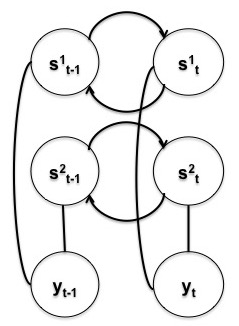
\includegraphics[width=4cm,height=4cm]{product}
\caption{Product of HMMs, P = $S^{1}$ x $S^2$}
\label{fig:product}
\end{figure*}


\subsection{Training the model by minimising contrastive divergence}
%Product of experts (PoE)\footnote{http://en.wikipedia.org/wiki/Product\_of\_experts} is a technique that models probability distribution by combining the output from several simpler distributions. It is defined by the following formula:\\
% Write the formula and explain it. Explain Gibbs Sampling

To fit the model to the data, we need to maximize the likelihood of the dataset or minimise the Kullback-Liebler divergence between the data distribution, $P^0$ (data distribution at time 0) and the equilibrium distribution over the visible variables, $P^\infty_\theta$ (fantasy data) which is obtained after prolonged Gibbs sampling as shown in equation~\ref{eq:KL}. 

\begin{eqnarray}
P^0 || P^\infty_\theta = \sum_{d}P^0 (d)logP^0(d) - \sum_{d}P^0 (d)logP^\infty_\theta(d) \label{eq:KL} \\
P^0 || P^\infty_\theta = -H(P^0) - \langle log P^\infty_\theta \rangle_{P^{0}}
\end{eqnarray}

where $||$ represents Kullback-Leibler divergence, d is the data vector in discrete space, $\theta_m$ is all the parameters of individual model m, $P^0$ is the data distribution at time $0$, H($P^0$) represents the entropy which is ignored during optimisation as $P^0$ does not depend on the parameters of the model, angle brackets denote the expectation over the distribution specified by the subscript.
In Gibbs sampling, each variable draws a sample from its posterior distribution given the current states of the other variables. The hidden states of all the models are conditionally independent given the data and hence can be parallel updated as shown in Figure~\ref{fig:gibbs}. At time t=0, the observed variables represent a data vector, d and the hidden variables, s of all the models are updated in parallel with samples from their posterior distribution given the observed variables, y. At time 1, the visible variables are updated to generate a reconstruction of the original data vector from the hidden variables and the hidden variables are again updated simultaneously. This prolonged sampling helps the Markov chain to converge to the equilibrium distribution which helps to attain the unbiased estimate of the gradient of the PoHMMs. But since the samples from the equilibrium state have high variance as they come from the entire model's distribution, it poses a difficulty in determining the estimate the derivative. Therefore, the optimisation is performed on the different objective function called contrastive divergence, defined in equation~\ref{eq:CD}. Contrastive divergence is the difference between $P^0 || P^\infty_\theta$ and $P^1_\theta || P^\infty_\theta$ where $P^1_\theta$ is the distribution over the one-step reconstruction of the data vectors generated by one full step of Gibbs sampling. The intuition behind using contrastive divergence is to leave the initial distribution $P^{0}$ over the visible variables unaltered and also the intractable expectation over $P^\infty_\theta$ gets cancelled out. Instead of comparing the initial and final derivatives, $P^0$ and $P^\infty_\theta$, the Markov chain is run for one full step and the parameters are updated to avoid the chain to wander away from the initial distribution on the first step. As $P^1$ is a step closer to $P^\infty$ which guarantees that $P^0 || P^\infty_\theta$ will always exceed $P^1_\theta || P^\infty_\theta$ ensuring a non negative value unless $P^0$ = $P^1_\theta$. If $P^0$ = $P^1_\theta$, then it implies that the chain is already in an equilibrium state, that is $P^0$ = $P^\infty_\theta$ hence making the value of contrastive divergence as $0$.

 \begin{figure*}[t]
\centering
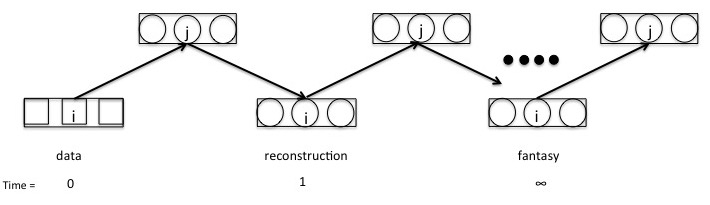
\includegraphics[width=12cm,height=4cm]{gibbs.jpg}
\caption{Visualization of Gibbs sampling}
\label{fig:gibbs}
\end{figure*}

\begin{eqnarray}
- \frac {\partial} {\partial\theta_{m}} (P^0 || P^\infty_\theta - P^1_\theta || P^\infty_\theta) = \langle \frac {\partial log f_{\theta_{m}}}{\partial \theta_m} \rangle_{P^0} \\
- \langle \frac {\partial log f_{\theta_{m}}}{\partial \theta_m} \rangle_{P^1_\theta} + \nonumber \frac{\partial{P^1_\theta}}{\partial\theta_m} \frac{\partial(P^1_\theta || P^\infty_\theta)}{\partial{P^1_\theta}}
 \label{eq:CD}
\end{eqnarray}
where log$f_{\theta_{m}}$ is a random variable that can also be written as $f_m$($D|\theta_m$) where D being a random variable corresponding to the data.
In equation~\ref{eq:CD}, the first two terms on the right hand side are tractable as it is easy to sample from $P^0$ and $P^1_\theta$ but the third term represents the effect on $P^1_\theta || P^\infty_\theta$ of the change of the step reconstruction caused by the change in the $\theta_m$. Extensive simulations show that it is small and rarely differs from the result of other two terms, hence can be safely ignored. Therefore in contrastive divergence, the parameters are learned according to the equation~\ref{eq:params}. To minimise the contrastive divergence by using a Markov chain that slowly mixes, we can use mixing techniques like weight decay that ensures that every possible visible vector has non zero probability given the latent variables.

\begin{eqnarray}
\Delta\theta_m \propto \langle \frac {\partial log f_{\theta_{m}}}{\partial \theta_m}\rangle_{P^0} - \langle \frac {\partial log f_{\theta_{m}}}{\partial \theta_m} \rangle_{P^1_\theta} \label{eq:params}
\end{eqnarray}

The contrastive divergence algorithm for training the PoHMM has the following steps:
\begin{enumerate}
\item Each model's gradient $\frac{\partial}{\partial\theta_m}$ $P(Y|\theta_m)$ ($\{y_t\}_{t=1}^T$ = Y is the visible variable) is calculated on a data point using forward backward algorithm.
\item A sample for each model is taken from the posterior distribution of paths through state space.
\item At each time step, the distributions are multiplied and renormalized together to get the reconstruction distribution.
\item A sample from the reconstruction distribution is drawn at each time step to get a reconstructed sequence. Each model's is gradient is computed on the new sequence $P(\hat Y|\theta_m)$
\item Parameters are updated as per equation~\ref{eq:params}

\end{enumerate}
%High dimensional distributions are approximated as a product of one dimensional distributions. The product of individual distributions which are uniguassian or multivariate guassian will also be multivariate guassian. If the individual models are more complicated and contain one or more hidden variables, multiplying their distributions together and renormalizing them can be very powerful. These individual models are called "experts".
%The product of experts produce sharper distribution than the individual distributions\cite{hinton2000}.

\subsection{Inference in PoHMM}

The main feature of PoHMMs is its undirected graphical modelling with no direct connection among the latent variables ($S^1_{t}$ and $S^2_{t}$) as they only interact indirectly via observed variables ($Y_{t}$). The hidden variables all the experts are rendered independent when conditioned on visible variables. So, if the inference in each of the constituent model is tractable then the inference in the product is also tractable. To generate a data point in this model, all the models in PoHMMs generate an observation and if they all generated the same point then it is accepted else they again generate an observation until all the models agree to it. Therefore all the models have some influence over the generated data. So, the inference determines the the probability that all the models would have taken in order to generate the given observation. 



\section{Applications using Product of HMM}
\label{poc}

\textbf{Aim}: In this section we demonstrate how PoHMMs can be used to model data streams and perform load forecasting. Proof-of-concepts are provided on two data sets - REDD\footnote{http://redd.csail.mit.edu/} and on the energy data collected from faculty housing at IIIT Delhi.
%To represent streams of energy consumption data from $n$\footnote{n=2} appliances by product of $k$ HMMs.

\subsection{Data Description} 
\begin{itemize}
\item \textbf{Dataset 1:} The Reference Energy Disaggregation Data Set (REDD) contains power consumption data from real homes, for the whole house as well as for each individual circuit in
the house (labeled by the main type of appliance on that circuit). %It is intended for use in developing disaggregation methods, which can predict, from only the whole-home signal, which devices are being used.
The REDD data set contains two main types of home electricity data: high-frequency current/voltage waveform data of the two power mains (as well as the voltage signal for a single phase), and lower-frequency power data including the mains and individual, labeled circuits in the house. 
%The main directory consists of several house directories, each of which contain all the power readings for a single house.  Each house subdirectory consists of a labels and channels files. The labels file helps in matching the channel number with the device name. Each channel file has two columns containing UTC timestamps (as integers) and power readings (recording the apparent power of the circuit) for the channel.
Experiments reported here use `house 2' data from REDD. This dataset has $318759$ records and $2$ columns. We randomly sample $300$ records for our initial experiment.
%The time series data of the microwave, dryer, kitchen$\_2$ and refrigerator are plotted below in Figures~\ref{fig:micro}, ~\ref{fig:washer}, ~\ref{fig:kitchen2}, ~\ref{fig:refri}. 
\subsubsection{Implementation Details}
The implementation of the product of hidden Markov model is obtained from Iain Murray's website\footnote{\label{link}http://homepages.inf.ed.ac.uk/imurray2/code/}. It implements the technique described in paper \cite{hinton2000}.
%Time series data from two appliances are represented as product of $k$ HMMs. It has $11$ channels where each channel corresponds to the following appliance, 1. mains1, 2. mains2, 3. kitchen 1, 4. lighting, 5. stove, 6. microwave, 7. washer dryer, 8. kitchen 2, 9. refrigerator, 10. dishwasher, 11. disposal


\item \textbf{Dataset 2:} This data represents the energy consumed by the IIIT Delhi's faculty housing building. As a part of research, a team from the institute has installed various temperature, light and motion sensors to perform real world studies and to analyse user preferences for energy conservation. For our analysis, we selected $1$ month's historical data ranging from 01-01-2014, 00:01 hours to 31-01-2014, 23:59 hours. The two smart meters installed, captured data from all the $12$ floors. The first meter records readings from ground to $5$th floor generating one stream of data and the second meter generates a stream from $6$th to $11$th. Both these streams are aggregated to obtain the aggregated load of the housing building. The dataset includes timestamp and power consumed in watts. There are $84133$ records in this dataset. We also have the total energy consumed by the faculty housing building which would serve as the ground truth to compare the aggregated load using PoHMMs.
%Time series data from two streams are modelled as a product of $k$ HMMs. 


\begin{figure*}[t]
\centering
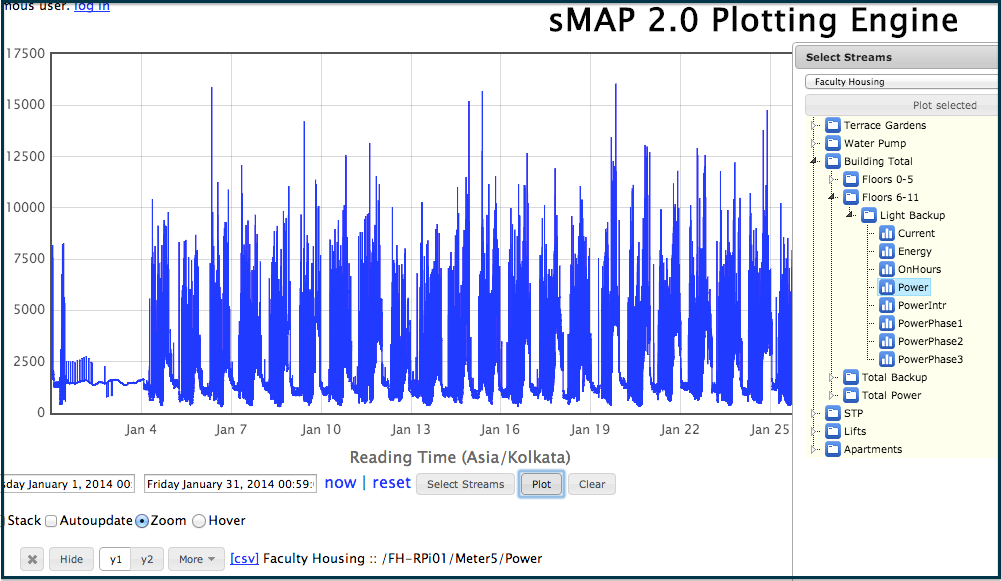
\includegraphics[width=0.8\textwidth,height=0.35\textheight]{./screenshot}
\caption{Screen shot of the tool that is used to download the energy data of the institute collected over the period of time.}
\label{fig:screenshot}
\end{figure*}


%\item \textbf{ Time Series :} The time series data of the microwave, dryer, kitchen$\_2$ and refrigerator are plotted below in Figures~\ref{fig:micro}, ~\ref{fig:washer}, ~\ref{fig:kitchen2}, ~\ref{fig:refri}.
%
%\begin{figure*}[t]
%\centering
%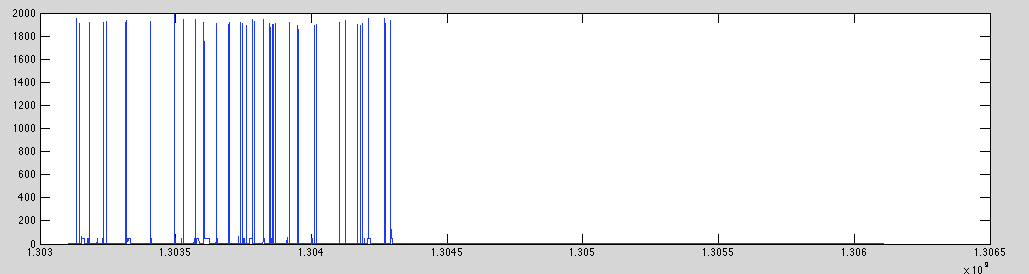
\includegraphics[width=1.0\textwidth,height=0.15\textheight]{channel_6.png}
%\caption{Microwave}
%\label{fig:micro}
%\end{figure*}
%
%\begin{figure*}[t]
%\centering
%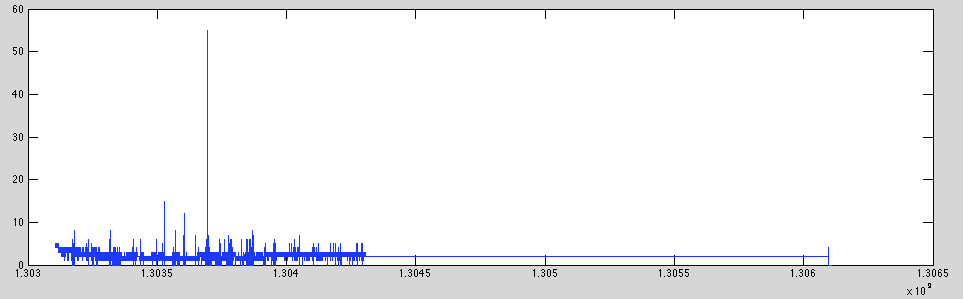
\includegraphics[width=1.0\textwidth,height=0.15\textheight]{channel_7.png}
%\caption{washer\_dryer}
%\label{fig:washer}
%\end{figure*}
%
%\begin{figure*}[th]
%\centering
%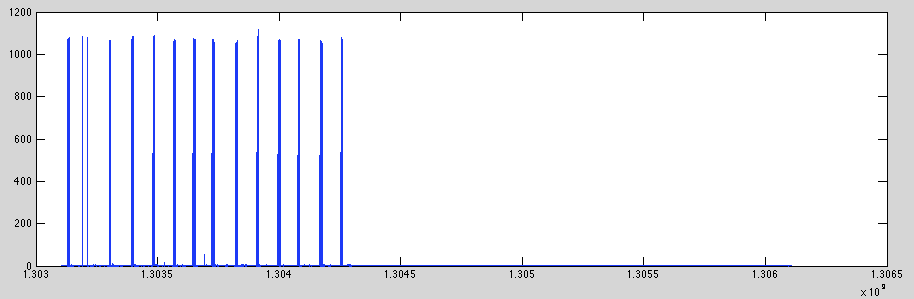
\includegraphics[width=1.0\textwidth,height=0.15\textheight]{channel_8.png}
%\caption{Kitchen\_2}
%\label{fig:kitchen2}
%\end{figure*}
%
%\begin{figure*}[th]
%\centering
%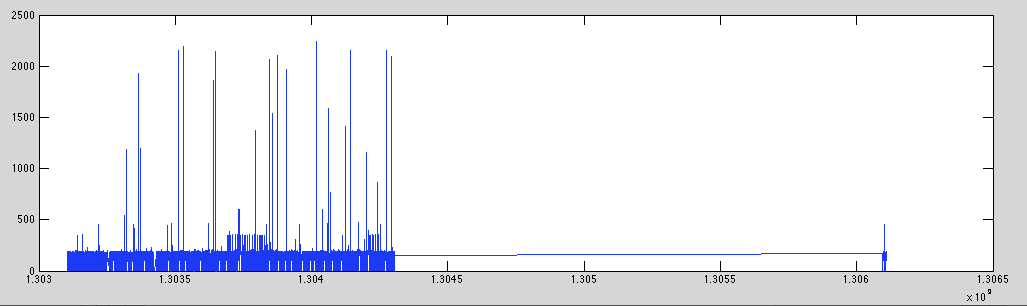
\includegraphics[width=1.0\textwidth,height=0.15\textheight]{channel_9.png}
%\caption{refrigerator}
%\label{fig:refri}
%\end{figure*}
%
%\item \textbf{Code } The implementation of the product of experts model is obtained from Iain Murray's website\footnote{\label{link}http://homepages.inf.ed.ac.uk/imurray2/code/}. It implements the technique described in Geoff Hinton's paper \cite{hinton2000}. 
%
%\item \textbf{Additional details }
%Some additional details regarding experiments:
%\begin{enumerate}
%\item The product of HMMs model (PoHMM) minimizes ``contrastive divergence" as described in the paper \cite{hinton2000}. 
%\item The number of experts, $k$ used here is 15. This is set somewhat arbitrarily and needs to be experimented on.
%\item Learning rate is $\epsilon = \frac{1}{300}$.
%\end{enumerate}
 
\end{itemize}

\subsection{Problem Formulation}
The disparate energy data streams collects readings at different time scales. Each of the data stream is modelled as a HMM with cardinality $2$, that is either ON or OFF. The process of aggregating the energy data from different data streams is modelled through PoHMMs. 

%Different smart meters can send data points when they are collected resulting in inconsistent data including aggregating non-aligned time stamped readings, readings with missing values, repeated values, meter reset readings.
%We address the problem of learning from disparate data streams (with inconsistencies) by modelling streams as HMMs and the process of aggregating data at the base station as a Product of HMMs. This enables us to perform load forecasting using machine learning techniques.
Each energy data stream is used to train the model, till the time the objective function, that is contrastive divergence reaches a threshold value. Once the model is trained from a randomly sampled data stream, the parameters learned by the model %(mixing component of each unigauss, means of gaussian bits, log precisions of axis-aligned gaussian bits) 
are provided to the randomly sampled test set (total energy consumed data) to obtain the conditional probability distribution of the gaussians given the data. Similarly, all the data streams are used for training the model, and the parameters learned are then applied on the test set to obtain the conditional probability of the gaussians given the data. After all the data streams are used to obtain the probability distribution, we use the data stream that correspond to the total energy consumed from the house/ building to train the model and hence obtain the probability distribution P of the gaussians. These probability distributions are then compared with the product of the probability distributions Q obtained from the individual data streams. The evaluation of how well the learning has taken place is done by using a Kullback-Leibler divergence. KL divergence of two probability distributions P and Q, $D_{KL}$(P$\parallel$Q) is the measure of information lost when Q is used to approximate P. %Here, P is the real data and Q is a fantasy data. The two probability distributions in the REDD example refer to the expert probabilities in real and fantasy data. 
%The learned parameters from the training are fitted to the fantasy data to measure the information lost when fantasy data is used to approximate real data.


%\subsection{Experimental Setup}
%%Experiments are performed on the REDD which contains $9$ appliances each containing $318759$ rows of energy consumption data. 
%Experiments are done into $4$ phases, in the first phase the number of data samples are varied corresponding to which the values of KL Divergence and convergence time are noted. In the second phase, the number of experts are varied keeping the best value of the sample from the first phase fixed. In the third phase, number of iterations are varied keeping the best values from above first two phases fixed. In the fourth part, the no. of appliances to be aggregated are varied.

%\begin{table*}[htdp]
%\begin{center}
%\begin{tabular}{| c | c | c | c |}
%\hline
%Samples & $KL Div$ & $Iterations$& $T(sec)$ \\
%\hline
%300 & 2.4864 & 18600 & 186.212 $\pm$9.087  \\
%500 & 0.6761 & 10200 & 106.564 $\pm$10.046 \\
%1000 & 1.1088 & 11200 & 158.521 $\pm$1.97  \\
%1500 & 3.8829 & 5300 & 92.896 $\pm$8.075  \\
%2000 & 1.8686 & 6900 & 130.98 $\pm$1.932 \\
%2500 & 0.4733 & 9900 & 215.563 $\pm$ 2.471 \\
%3000 & 2.8204 & 11000 & 258.213 $\pm1.918$ \\
%3500 & 1.2332 & 7900 & 204.661 $\pm$1.713 \\
%4000 & 0.8959 & 10400 & 292.666 $\pm$0.619 \\
%4500 & 1.1118 & 7200 & 222.558 $\pm$1.967 \\
%8000 & 6.392 & 8100 & 381.635 $\pm$2.952  \\
%10000 & 8.276 & 10500 & 887.932 $\pm$13.824  \\
%15000 & 0.7201 & 9400 & 1368.514 $\pm$13.605  \\
%\hline
%\end{tabular}
%\end{center}
%\caption{Effect of varying samples (REDD)}
%\label{table:sample1}
%\end{table*}



\begin{table*}[htdp]
\parbox{.43\linewidth}{
\centering
\begin{tabular}{| c | c | c | c |}
\hline
Samples & $KL Div$ & $Iterations$& $T(sec)$ \\
\hline
300 & 2.4864 & 18600 & 186.212 $\pm$9.087  \\
500 & 0.6761 & 10200 & 106.564 $\pm$10.046 \\
1000 & 1.1088 & 11200 & 158.521 $\pm$1.97  \\
1500 & 3.8829 & 5300 & 92.896 $\pm$8.075  \\
2000 & 1.8686 & 6900 & 130.98 $\pm$1.932 \\
2500 & 0.4733 & 9900 & 215.563 $\pm$ 2.471 \\
3000 & 2.8204 & 11000 & 258.213 $\pm1.918$ \\
3500 & 1.2332 & 7900 & 204.661 $\pm$1.713 \\
4000 & 0.8959 & 10400 & 292.666 $\pm$0.619 \\
4500 & 1.1118 & 7200 & 222.558 $\pm$1.967 \\
8000 & 6.392 & 8100 & 381.635 $\pm$2.952  \\
10000 & 8.276 & 10500 & 887.932 $\pm$13.824  \\
15000 & 0.7201 & 9400 & 1368.514 $\pm$13.605  \\
\hline
\end{tabular}
\caption{Effect of varying samples (REDD)}
\label{table:sample1}}
\hfill
\parbox{.43\linewidth}{
\centering
\begin{tabular}{| c | c | c | c |}
\hline
Samples & $KL Div(e-04)$  & $Iterations$ & $T(sec)$\\
\hline
100 & 0.26219 & 45100 & 257  \\
300 & 0.19753 & 43200 & 222 \\
500 & 0.55493 & 44800 & 260  \\
700 & 0.32847 & 44000 & 249 \\
900 & 3.9486 & 42600 & 221  \\
1100 & 4.9274 & 44700 & 317  \\
1300 & 3.0425 & 43100 & 276 \\
1500 &  3.1128 & 44400 & 303 \\
2000 & 1.9192 & 44400 & 306 \\
2500 & 1.7122 & 44100 & 370 \\
3000 & 1.4686 & 43300 & 331 \\
3500 & 1.2663 & 43200 & 370  \\
4000 & 1.0793 & 43200 & 403  \\
\hline
\end{tabular}
\caption{Effect of varying samples (housing data)}
\label{table:sample2}}
\end{table*}






\subsection{Empirical Results}
In both the datasets, experiments are performed by tuning some parameters and keeping some fixed.
In case of REDD, Tables~\ref{table:sample1},~\ref{table:threshold1} and \ref{table:hmm1} show the effect of varying data samples, threshold and no. of HMMs on KL divergence. In Table \ref{table:sample1}, data samples are randomly selected from the dataset, KL divergence is chosen as the performance metric, iterations are performed to obtain the samples from the equilibrium distribution by using Gibbs sampler on the hidden and visible variables and the average time taken (sec) with the standard deviation on three such iterations is noted in the last column.

 In case of faculty housing dataset, Tables~\ref{table:sample2},~\ref{table:threshold2} and \ref{table:hmm2} show the effect of varying data samples, threshold and no. of HMMs on the KL divergence. As per table \ref{table:sample1} and \ref{table:sample2}, the relation between no. of samples and KL divergence was observed, the best performance was attained when $2500$ and $300$ samples were randomly chosen from the REDD and faculty housing dataset respectively. In table \ref{table:threshold1} and \ref{table:threshold2}, there is an indirect relationship between threshold and KL divergence value, that is lower the threshold, higher the KL divergence. 
%Similarly, the relationship between threshold values and iterations/time taken is indirect.
When all the appliances in `house 2' (total appliances are $9$) of REDD are used in PoHMMs and similarly when both the data streams of faculty housing building are aggregated, the performance is at its best as can be seen in Table \ref{table:hmm1} and \ref{table:hmm2}. The value of KL divergence is minimum when the energy data from all the appliances are aggregated and tested against total energy data. % keeping the threshold value fixed at $0.1$ and no. of appliances fixed at $15$.

%Experiments are done into $4$ phases, in the first phase the number of data samples are varied corresponding to which the values of KL Divergence and convergence time are noted. In the second phase, the number of experts are varied keeping the best value of the sample from the first phase fixed. In the third phase, number of iterations are varied keeping the best values from above first two phases fixed. In the fourth part, the no. of appliances to be aggregated are varied.

%The evaluation of how well the learning has taken place is done by using a Kullback-Leibler divergence. KL divergence of P from Q, $D_{KL}$(P$\parallel$Q) is the measure of information lost when Q is used to approximate P. Here, P is the real data and Q is a fantasy data. The two probability distributions in the REDD example refer to the expert probabilities in real and fantasy data. The learned parameters from the training are fitted to the fantasy data to measure the information lost when fantasy data is used to approximate real data.


\begin{table*}[htdp]
\parbox{.57\linewidth}{
\centering
\begin{tabular}{| c | c | c | c |}
\hline
Threshold & $KL Div$ & $Iterations$ & $T(sec)$  \\
\hline
.1 & 0.473 & 9900 & 210.6 $\pm$1.493 \\
.05 & 0.443 & 10900 & 240.607$\pm$2.436 \\
.01 & 0.454 & 18000 & 431.536 $\pm$14.509 \\
.005 & 0.509 & 49800 & 1167.243 $\pm$43.412 \\
\hline
\end{tabular}
\caption{Effect of varying threshold (REDD)}
\label{table:threshold1}
}
\hfill
\parbox{.57\linewidth}{
\centering
\begin{tabular}{| c | c | c | c |}
\hline
Threshold & $KL Div(e-04)$ & $Iterations$& $T(sec)$ \\
\hline
0.9 & 0.768 & 49300 & 153.67 $\pm$13.57  \\
0.8 & 0.768 & 49300 & 190.3 $\pm$34.35 \\
0.7 & 0.769 & 49400 &  193.67$\pm$31.64  \\
0.6 & 0.792 & 49500 & 218.3 $\pm$43.93  \\
0.5 & 0.793 & 49600 & 250.67$\pm$3.51  \\
0.4 & 0.854 & 49600 & 191$\pm$35.55  \\
\hline
\end{tabular}
\caption{Effect of varying threshold (housing data)}
\label{table:threshold2}
}
\end{table*}



\begin{table*}[htdp]
\parbox{.45\linewidth}{
\centering
\begin{tabular}{| c | c | c | c |}
\hline
HMMs & $KL Div$ & $Iterations$ & $T(sec)$  \\
\hline
3 & 5.559  & 10700 & 233.664 $\pm$0.579 \\
4 & 0.188 & 19900 & 465.634 $\pm$5.275  \\
5 & .432  & 13400 & 338.416 $\pm$3.988  \\
6 & 8.736  & 28100 & 606.062 $\pm$7.534 \\
7 & 5.054  & 17300 & 411.457 $\pm$10.051\\
8 & 0.436 & 10700 & 260.544 $\pm$27.862 \\
9 & 0.15 & 20600 & 474.579 $\pm$14.619 \\
\hline
\end{tabular}
\caption{Effect of varying HMMs (REDD)}
\label{table:hmm1}}
\hfill
\parbox{.45\linewidth}{
\centering
\begin{tabular}{| c | c | c | c |}
\hline
HMMs & $KL Div (e-04)$ & Iterations & $T(sec)$\\
\hline
2 & 0 & 49200 & 233.33 $\pm$7.23 \\
3 & 0.81 & 49200 & 237.67 $\pm$10.59 \\
5 & 0.77 & 49300 & 242.33 $\pm$3 \\
10 & 2.12 & 49300 & 228.33 $\pm$46.23 \\
15 & 2.55 & 49300 & 269.33 $\pm$17.61 \\
20 & 2.23 & 49300 & 305.66 $\pm$2.08  \\
25 & 2.19 & 49300 & 302.33 $\pm$8 \\
30 & 2.24 & 49300 & 336.33 $\pm$9.5 \\
35 & 1.94 & 49300 & 331.33 $\pm$9 \\
\hline
\end{tabular}
\caption{Effect of varying HMMs (housing data)}
\label{table:hmm2}
}
\end{table*}







\section{Conclusion}
\label{conclusion}

In this paper, we are solving the problem of load aggregation (energy consumption) for disparate energy data sources using the ensemble based learning technique called Product of HMMs. Several challenges are faced while computing the aggregated energy, few of which include non-aligned timestamp readings, missing values, meter reset readings. This technique produces the combined probability distributions of several simpler distributions and then renormalizes this output. The optimisation problem is to minimise the contrastive divergence between the two probability distributions of the data at time $0$ and the data at time $1$ (one-step reconstruction using gibbs sampling). The evaluation of the algorithm is done by computing the KL divergence between the product of the energy data distributions and the total energy data distribution. From the results shown in table \ref{table:hmm1} and \ref{table:hmm2}, we can see that the algorithm has performed best when the number of appliances (REDD) reached the actual number of appliances ($9$) in the house and the number of data streams in case of housing data reached the actual number of streams ($2$) used in the 12 floor faculty housing data. Therefore, this signifies that this algorithm is applicable for this kind of application and can be used for load forecasting.


% use section* for acknowledgement

\section*{Acknowledgment}
The authors would like to thank $EMC^2$ for supporting this research through grant number JRA092014-Q3-5.
%
%
%The authors would like to thank...



\nocite{CarrieArmel2013213,eps272990,NIPS2010,Rabiner,SS97a,Kawamoto,Diane,Klopfert,Ghahramani,Felice,Shen,taban,Albert,wijaya2014consumer,Zhang,Daneshi,bassi,samuel,Falvo,Bakirtzis,Chen,Chow,DisaggregationHSMM,KolterJ12,KolterF11,BLTJ:BLTJ21650,Heinzelman00energy,Taylor,NYAS:NYAS5921,
Wijaya,5620917,1626400,mckerracher,hinton2000,aistats,fhmm,andrew}

% trigger a \newpage just before the given reference
% number - used to balance the columns on the last page
% adjust value as needed - may need to be readjusted if
% the document is modified later
%\IEEEtriggeratref{8}
% The "triggered" command can be changed if desired:
%\IEEEtriggercmd{\enlargethispage{-5in}}

% references section

% can use a bibliography generated by BibTeX as a .bbl file
% BibTeX documentation can be easily obtained at:
% http://www.ctan.org/tex-archive/biblio/bibtex/contrib/doc/
% The IEEEtran BibTeX style support page is at:
% http://www.michaelshell.org/tex/ieeetran/bibtex/
\bibliographystyle{llncs}
% argument is your BibTeX string definitions and bibliography database(s)
%\bibliography{IEEEabrv,IEEEexample}
\bibliography{typeinst}



%\subsection{Checking the PDF File}
%
%Kindly assure that the Contact Volume Editor is given the name and email
%address of the contact author for your paper. The Contact Volume Editor
%uses these details to compile a list for our production department at
%SPS in India. Once the files have been worked upon, SPS sends a copy of
%the final pdf of each paper to its contact author. The contact author is
%asked to check through the final pdf to make sure that no errors have
%crept in during the transfer or preparation of the files. This should
%not be seen as an opportunity to update or copyedit the papers, which is
%not possible due to time constraints. Only errors introduced during the
%preparation of the files will be corrected.
%
%This round of checking takes place about two weeks after the files have
%been sent to the Editorial by the Contact Volume Editor, i.e., roughly
%seven weeks before the start of the conference for conference
%proceedings, or seven weeks before the volume leaves the printer's, for
%post-proceedings. If SPS does not receive a reply from a particular
%contact author, within the timeframe given, then it is presumed that the
%author has found no errors in the paper. The tight publication schedule
%of LNCS does not allow SPS to send reminders or search for alternative
%email addresses on the Internet.
%
%In some cases, it is the Contact Volume Editor that checks all the final
%pdfs. In such cases, the authors are not involved in the checking phase.
%
%\subsection{Additional Information Required by the Volume Editor}
%
%If you have more than one surname, please make sure that the Volume Editor
%knows how you are to be listed in the author index.
%
%\subsection{Copyright Forms}
%
%The copyright form may be downloaded from the ``For Authors"
%(Information for LNCS Authors) section of the LNCS Website:
%\texttt{www.springer.com/lncs}. Please send your signed copyright form
%to the Contact Volume Editor, either as a scanned pdf or by fax or by
%courier. One author may sign on behalf of all of the other authors of a
%particular paper. Digital signatures are acceptable.
%
%\section{Paper Preparation}
%
%Springer provides you with a complete integrated \LaTeX{} document class
%(\texttt{llncs.cls}) for multi-author books such as those in the LNCS
%series. Papers not complying with the LNCS style will be reformatted.
%This can lead to an increase in the overall number of pages. We would
%therefore urge you not to squash your paper.
%
%Please always cancel any superfluous definitions that are
%not actually used in your text. If you do not, these may conflict with
%the definitions of the macro package, causing changes in the structure
%of the text and leading to numerous mistakes in the proofs.
%
%If you wonder what \LaTeX{} is and where it can be obtained, see the
%``\textit{LaTeX project site}'' (\url{http://www.latex-project.org})
%and especially the webpage ``\textit{How to get it}''
%(\url{http://www.latex-project.org/ftp.html}) respectively.
%
%When you use \LaTeX\ together with our document class file,
%\texttt{llncs.cls},
%your text is typeset automatically in Computer Modern Roman (CM) fonts.
%Please do
%\emph{not} change the preset fonts. If you have to use fonts other
%than the preset fonts, kindly submit these with your files.
%
%Please use the commands \verb+\label+ and \verb+\ref+ for
%cross-references and the commands \verb+\bibitem+ and \verb+\cite+ for
%references to the bibliography, to enable us to create hyperlinks at
%these places.
%
%For preparing your figures electronically and integrating them into
%your source file we recommend using the standard \LaTeX{} \verb+graphics+ or
%\verb+graphicx+ package. These provide the \verb+\includegraphics+ command.
%In general, please refrain from using the \verb+\special+ command.
%
%Remember to submit any further style files and
%fonts you have used together with your source files.
%
%\subsubsection{Headings.}
%
%Headings should be capitalized
%(i.e., nouns, verbs, and all other words
%except articles, prepositions, and conjunctions should be set with an
%initial capital) and should,
%with the exception of the title, be aligned to the left.
%Words joined by a hyphen are subject to a special rule. If the first
%word can stand alone, the second word should be capitalized.
%
%Here are some examples of headings: ``Criteria to Disprove
%Context-Freeness of Collage Language", ``On Correcting the Intrusion of
%Tracing Non-deterministic Programs by Software", ``A User-Friendly and
%Extendable Data Distribution System", ``Multi-flip Networks:
%Parallelizing GenSAT", ``Self-determinations of Man".
%
%\subsubsection{Lemmas, Propositions, and Theorems.}
%
%The numbers accorded to lemmas, propositions, and theorems, etc. should
%appear in consecutive order, starting with Lemma 1, and not, for
%example, with Lemma 11.
%
%\subsection{Figures}
%
%For \LaTeX\ users, we recommend using the \emph{graphics} or \emph{graphicx}
%package and the \verb+\includegraphics+ command.
%
%Please check that the lines in line drawings are not
%interrupted and are of a constant width. Grids and details within the
%figures must be clearly legible and may not be written one on top of
%the other. Line drawings should have a resolution of at least 800 dpi
%(preferably 1200 dpi). The lettering in figures should have a height of
%2~mm (10-point type). Figures should be numbered and should have a
%caption which should always be positioned \emph{under} the figures, in
%contrast to the caption belonging to a table, which should always appear
%\emph{above} the table; this is simply achieved as matter of sequence in
%your source.
%
%Please center the figures or your tabular material by using the \verb+\centering+
%declaration. Short captions are centered by default between the margins
%and typeset in 9-point type (Fig.~\ref{fig:example} shows an example).
%The distance between text and figure is preset to be about 8~mm, the
%distance between figure and caption about 6~mm.
%
%To ensure that the reproduction of your illustrations is of a reasonable
%quality, we advise against the use of shading. The contrast should be as
%pronounced as possible.
%
%If screenshots are necessary, please make sure that you are happy with
%the print quality before you send the files.

%\begin{figure}
%\centering
%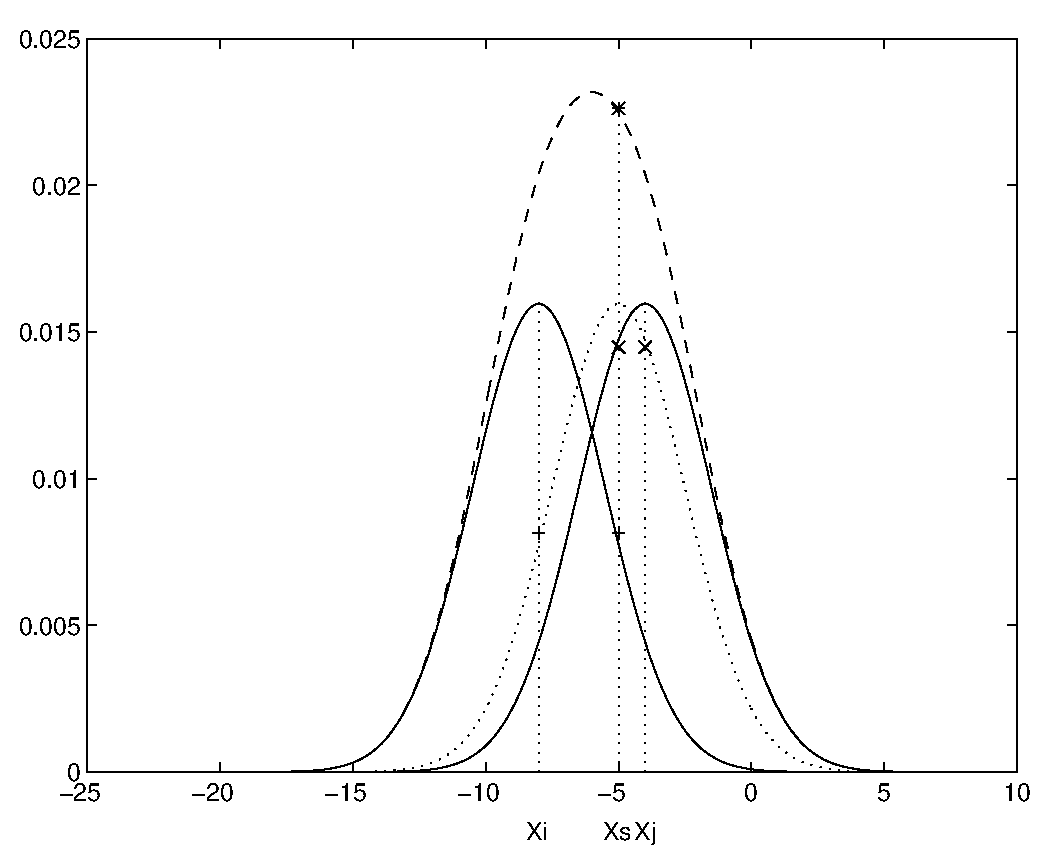
\includegraphics[height=6.2cm]{/Users/meghagupta/Downloads/eijkel2}
%\caption{One kernel}
%\label{fig:example}
%\end{figure}

%Please define figures (and tables) as floating objects. Please avoid
%using optional location parameters like ``\verb+[h]+" for ``here".
%
%\paragraph{Remark 1.}
%
%In the printed volumes, illustrations are generally black and white
%(halftones), and only in exceptional cases, and if the author is
%prepared to cover the extra cost for color reproduction, are colored
%pictures accepted. Colored pictures are welcome in the electronic
%version free of charge. If you send colored figures that are to be
%printed in black and white, please make sure that they really are
%legible in black and white. Some colors as well as the contrast of
%converted colors show up very poorly when printed in black and white.
%
%\subsection{Formulas}
%
%Displayed equations or formulas are centered and set on a separate
%line (with an extra line or halfline space above and below). Displayed
%expressions should be numbered for reference. The numbers should be
%consecutive within each section or within the contribution,
%with numbers enclosed in parentheses and set on the right margin --
%which is the default if you use the \emph{equation} environment, e.g.,
%\begin{equation}
%  \psi (u) = \int_{o}^{T} \left[\frac{1}{2}
%  \left(\Lambda_{o}^{-1} u,u\right) + N^{\ast} (-u)\right] dt \;  .
%\end{equation}
%
%Equations should be punctuated in the same way as ordinary
%text but with a small space before the end punctuation mark.
%
%\subsection{Footnotes}
%
%The superscript numeral used to refer to a footnote appears in the text
%either directly after the word to be discussed or -- in relation to a
%phrase or a sentence -- following the punctuation sign (comma,
%semicolon, or period). Footnotes should appear at the bottom of
%the
%normal text area, with a line of about 2~cm set
%immediately above them.\footnote{The footnote numeral is set flush left
%and the text follows with the usual word spacing.}
%
%\subsection{Program Code}
%
%Program listings or program commands in the text are normally set in
%typewriter font, e.g., CMTT10 or Courier.
%
%\medskip
%
%\noindent
%{\it Example of a Computer Program}
%\begin{verbatim}
%program Inflation (Output)
%  {Assuming annual inflation rates of 7%, 8%, and 10%,...
%   years};
%   const
%     MaxYears = 10;
%   var
%     Year: 0..MaxYears;
%     Factor1, Factor2, Factor3: Real;
%   begin
%     Year := 0;
%     Factor1 := 1.0; Factor2 := 1.0; Factor3 := 1.0;
%     WriteLn('Year  7% 8% 10%'); WriteLn;
%     repeat
%       Year := Year + 1;
%       Factor1 := Factor1 * 1.07;
%       Factor2 := Factor2 * 1.08;
%       Factor3 := Factor3 * 1.10;
%       WriteLn(Year:5,Factor1:7:3,Factor2:7:3,Factor3:7:3)
%     until Year = MaxYears
%end.
%\end{verbatim}
%%
%\noindent
%{\small (Example from Jensen K., Wirth N. (1991) Pascal user manual and
%report. Springer, New York)}
%
%\subsection{Citations}
%
%For citations in the text please use
%square brackets and consecutive numbers: \cite{jour}, \cite{lncschap},
%\cite{proceeding1} -- provided automatically
%by \LaTeX 's \verb|\cite| \dots\verb|\bibitem| mechanism.
%
%\subsection{Page Numbering and Running Heads}
%
%There is no need to include page numbers. If your paper title is too
%long to serve as a running head, it will be shortened. Your suggestion
%as to how to shorten it would be most welcome.
%
%\section{LNCS Online}
%
%The online version of the volume will be available in LNCS Online.
%Members of institutes subscribing to the Lecture Notes in Computer
%Science series have access to all the pdfs of all the online
%publications. Non-subscribers can only read as far as the abstracts. If
%they try to go beyond this point, they are automatically asked, whether
%they would like to order the pdf, and are given instructions as to how
%to do so.
%
%Please note that, if your email address is given in your paper,
%it will also be included in the meta data of the online version.
%
%\section{BibTeX Entries}
%
%The correct BibTeX entries for the Lecture Notes in Computer Science
%volumes can be found at the following Website shortly after the
%publication of the book:
%\url{http://www.informatik.uni-trier.de/~ley/db/journals/lncs.html}
%
%\subsubsection*{Acknowledgments.} The heading should be treated as a
%subsubsection heading and should not be assigned a number.
%
%\section{The References Section}\label{references}
%
%In order to permit cross referencing within LNCS-Online, and eventually
%between different publishers and their online databases, LNCS will,
%from now on, be standardizing the format of the references. This new
%feature will increase the visibility of publications and facilitate
%academic research considerably. Please base your references on the
%examples below. References that don't adhere to this style will be
%reformatted by Springer. You should therefore check your references
%thoroughly when you receive the final pdf of your paper.
%The reference section must be complete. You may not omit references.
%Instructions as to where to find a fuller version of the references are
%not permissible.
%
%We only accept references written using the latin alphabet. If the title
%of the book you are referring to is in Russian or Chinese, then please write
%(in Russian) or (in Chinese) at the end of the transcript or translation
%of the title.
%
%The following section shows a sample reference list with entries for
%journal articles \cite{jour}, an LNCS chapter \cite{lncschap}, a book
%\cite{book}, proceedings without editors \cite{proceeding1} and
%\cite{proceeding2}, as well as a URL \cite{url}.
%Please note that proceedings published in LNCS are not cited with their
%full titles, but with their acronyms!
%
%\begin{thebibliography}{4}
%
%\bibitem{jour} Smith, T.F., Waterman, M.S.: Identification of Common Molecular
%Subsequences. J. Mol. Biol. 147, 195--197 (1981)
%
%\bibitem{lncschap} May, P., Ehrlich, H.C., Steinke, T.: ZIB Structure Prediction Pipeline:
%Composing a Complex Biological Workflow through Web Services. In: Nagel,
%W.E., Walter, W.V., Lehner, W. (eds.) Euro-Par 2006. LNCS, vol. 4128,
%pp. 1148--1158. Springer, Heidelberg (2006)
%
%\bibitem{book} Foster, I., Kesselman, C.: The Grid: Blueprint for a New Computing
%Infrastructure. Morgan Kaufmann, San Francisco (1999)
%
%\bibitem{proceeding1} Czajkowski, K., Fitzgerald, S., Foster, I., Kesselman, C.: Grid
%Information Services for Distributed Resource Sharing. In: 10th IEEE
%International Symposium on High Performance Distributed Computing, pp.
%181--184. IEEE Press, New York (2001)
%
%\bibitem{proceeding2} Foster, I., Kesselman, C., Nick, J., Tuecke, S.: The Physiology of the
%Grid: an Open Grid Services Architecture for Distributed Systems
%Integration. Technical report, Global Grid Forum (2002)
%
%\bibitem{url} National Center for Biotechnology Information, \url{http://www.ncbi.nlm.nih.gov}
%
%\end{thebibliography}
%
%
%\section*{Appendix: Springer-Author Discount}
%
%LNCS authors are entitled to a 33.3\% discount off all Springer
%publications. Before placing an order, the author should send an email, 
%giving full details of his or her Springer publication,
%to \url{orders-HD-individuals@springer.com} to obtain a so-called token. This token is a
%number, which must be entered when placing an order via the Internet, in
%order to obtain the discount.
%
%\section{Checklist of Items to be Sent to Volume Editors}
%Here is a checklist of everything the volume editor requires from you:
%
%
%\begin{itemize}
%\settowidth{\leftmargin}{{\Large$\square$}}\advance\leftmargin\labelsep
%\itemsep8pt\relax
%\renewcommand\labelitemi{{\lower1.5pt\hbox{\Large$\square$}}}
%
%\item The final \LaTeX{} source files
%\item A final PDF file
%\item A copyright form, signed by one author on behalf of all of the
%authors of the paper.
%\item A readme giving the name and email address of the
%corresponding author.
%\end{itemize}



\end{document}
